\section{Implementation}
\label{sec:implementation}

In this section, we present our implementation of the MapReduce framework. We first discuss the design objectives in Section~\ref{sec:design}, followed by the features of our framework in Section~\ref{sec:features}. We then describe the architecture of our framework in Section~\ref{sec:details}.

\subsection{Design Objectives}
\label{sec:design}

Our implementation of the MapReduce framework aims to achieve the following Design Objectives (DOs):

\begin{itemize}
    \item \textbf{DO1: Ease of Use.} This is of prime importance, as the framework should be easy to use and require minimal configuration to run MapReduce jobs. Like Hadoop, the framework should provide several simple APIs for users to define their map and reduce functions.
    \item \textbf{DO2: High Efficiency.} The framework should be efficient in terms of resource utilization, task scheduling, and data processing to minimize job completion time. This can be achieved by leveraging in-memory operations to minimize disk I/O overhead.
    \item \textbf{DO3: Fault Tolerance.} The framework should be adaptive to failures, such as worker node crashes, network failures, or data corruption. It should be able to recover from such failures and continue processing the job without data loss. In other words, if a worker node fails, the master node should accurately detect the failure and be able to reassign the task to another worker node.
    % \item \textbf{DO4: Extensibility.} The framework should be able to scale efficiently across multiple nodes in a distributed environment. Users are capable of adding new worker nodes to the cluster to increase the processing capacity, dynamically adjusting the number of mappers and reducers to optimize the performance.
\end{itemize}

\subsection{Features}
\label{sec:features}

In this part, we discuss the implementation details of our MapReduce framework. 

\textbf{DO1: MapReduce Interfaces.} We provide a simple and intuitive interface for users to define their map and reduce functions. Users can implement the \texttt{Mapper} and \texttt{Reducer} interfaces to define their map and reduce functions, respectively. The \texttt{Mapper} class provides a \texttt{map} method that takes an input key and value and emits intermediate key-value pairs, while the \texttt{Reducer} class provides a \texttt{reduce} method that takes an intermediate key and a list of values and emits the final output key-value pairs. To scale the framework to different types of data, both the input and output of the map and reduce functions are generic types.

\textbf{DO2: Communication Framework.} We adopt the Google Remote Procedure Call (gRPC) framework for communication between the master node and the worker nodes. gRPC is a high-performance, open-source RPC framework that provides communication between distributed systems, which can be used to define the service interfaces and generate client and server stubs in multiple programming languages, such as Java, Python, and Go. This communication framework ensures efficient and reliable communication between the master and worker nodes. In our implementation, tasks are sent from the master node to the worker nodes using gRPC, and the worker nodes send heartbeat messages to the master node to indicate their status. 

\textbf{DO3: Heartbeat Mechanism.} To detect worker node failures, we implement a heartbeat mechanism between the master node and the worker nodes. The worker nodes periodically send heartbeat messages to the master node to indicate that they are alive and functioning properly. If the master node does not receive a heartbeat message from a worker node within a specified timeout period, e.g., 1000 milliseconds, it marks the worker node as failed and reassigns its tasks to other worker nodes. Besides, users can easily distinguish failed worker nodes from the master node's logs. Overall, this mechanism ensures fault tolerance in the MapReduce framework and allows it to adapt to worker node failures.

% \textbf{DO4: Dynamic Scaling.} Our MapReduce framework supports dynamic scaling of the cluster by allowing users to add during the execution of a MapReduce job. When a new worker node joins the cluster, the master node detects the new node and assigns tasks to it based on the current load and task distribution. Similarly, when a worker node leaves the cluster, the master node redistributes the tasks to the remaining worker nodes to maintain load balance. This dynamic scaling capability allows the MapReduce framework to efficiently utilize the cluster resources and optimize the job performance.
 
\begin{figure*}
    \centering
    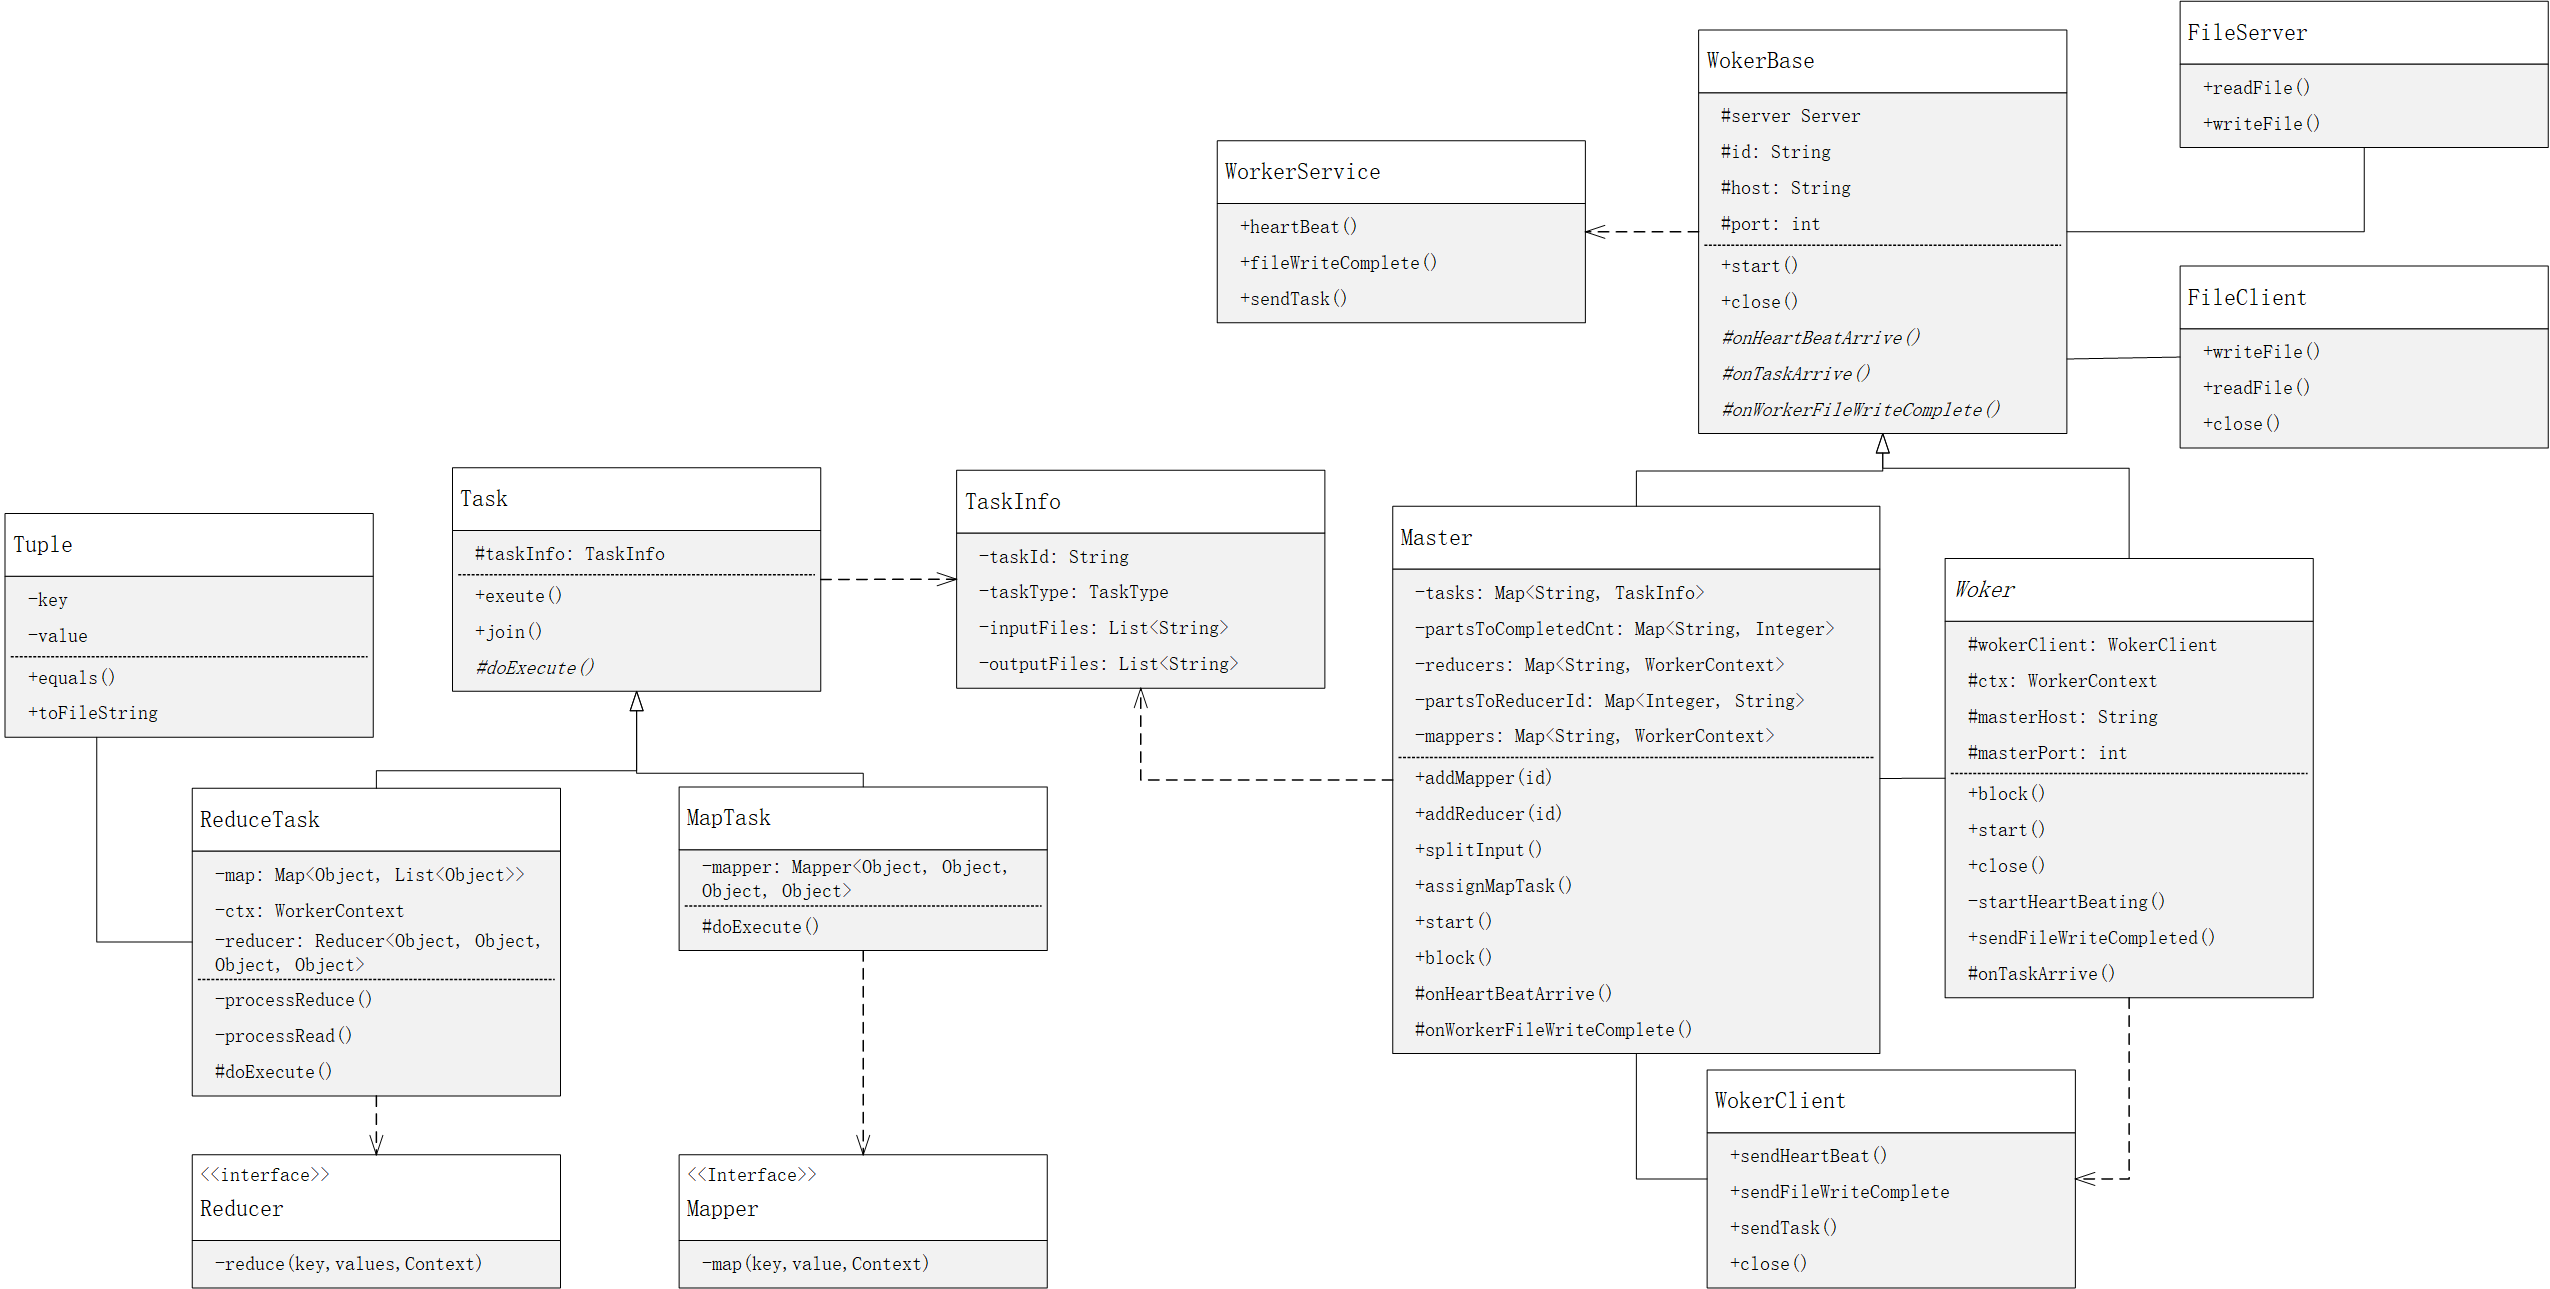
\includegraphics[width=1.0\textwidth]{class}
    \vspace{0.5em}
    \caption{Class diagram of our implemented MapReduce framework.}
    \label{fig:class}
\end{figure*}

\subsection{Implementation Details}
\label{sec:details}

In this part, we present the architecture of our implemented MapReduce framework. The class diagram of our framework is shown in Figure~\ref{fig:class}.

As illustrated in the figure, our MapReduce framework consists of several key components:

\begin{itemize}
    \item \textbf{Master:} The \texttt{Master} class is responsible for coordinating and managing tasks across the system. It tracks the state of tasks via a map (i.e., a HashMap), keeps track of completed parts (\texttt{partsToCompletedCnt()}), and assigns tasks to workers. The \texttt{Master} is also responsible for splitting input data (\texttt{splitInput()}) and distributing map tasks using methods like \texttt{assignMapTask()}. Communication with workers is handled via heartbeat signals (\texttt{onHeartBeatArrive()}) and file write completion events (\texttt{onWorkerFileWriteComplete()}).
    \item \textbf{Worker:} The \texttt{Worker} class serves as the executor of tasks assigned by the \texttt{Master}. Each worker communicates with the \texttt{Master} through its \texttt{WorkerClient} instance. The worker periodically sends heartbeat signals (\texttt{startHeartBeating()}) and notifies the \texttt{Master} when it completes file writes or receives a new task (\texttt{onTaskArrive()}). This ensures the \texttt{Master} remains aware of the worker’s status.
    \item \textbf{Task:} The \texttt{Task} class serves as an abstraction for different types of MapReduce tasks. It includes details about the task (\texttt{TaskInfo}) and defines methods for execution (\texttt{execute()}) and task synchronization (\texttt{join()}). The \texttt{Task} class is extended by \texttt{MapTask} and \texttt{ReduceTask} to implement specific MapReduce functionality. Both of these subclasses override the core execution logic defined in the \texttt{doExecute()} method.
    \item \textbf{MapTask and ReduceTask:} The \texttt{MapTask} handles the mapping phase, utilizing a \texttt{Mapper} instance to process key-value pairs. It operates on input data and generates intermediate key-value pairs. The \texttt{ReduceTask}, on the other hand, executes the reduce phase, using a \texttt{Reducer} instance to aggregate values associated with each key. Methods like \texttt{processReduce()} and \texttt{processRead()} manage the input and output of data during the reduce phase.
    \item \textbf{TaskInfo:} The \texttt{TaskInfo} class encapsulates metadata for a task, such as its unique identifier (\texttt{taskId()}), type (\texttt{taskType()}), input files (\texttt{inputFiles()}), and output files (\texttt{outputFiles()}). This class provides a structured way to manage task-related information across the system.
    \item \textbf{WorkerBase:}\texttt{WokerBase} defines the basic attributes shared by both \texttt{Master} and \texttt{Woker}. In addition, the \texttt{WokerBase} class provides several abstract event-handling functions. Among them, \texttt{onWorkerFileWriteComplete()} and \texttt{onHeartBeatArrive()} need to be implemented in the \texttt{Master} class because the master is responsible for monitoring the heartbeat of workers and receiving output files from workers. The \texttt{onTaskArrive()} function needs to be implemented in the worker class since the worker is responsible for receiving tasks.
    \item \textbf{WorerClient and WokerService:} \texttt{WorkerService} and \texttt{WorkerClient} are classes created to implement \texttt{gRPC} communication. WorkerService is a server-side class designed to handle requests, while WorkerClient is a client-side class used to send requests. The functions in WorkerService define how to respond to requests. A Worker periodically sends heartbeat signals to the Master using the \texttt{sendHeartBeat()} method of WorkerClient. When a task is completed, the Worker sends the result to the Master via the \texttt{sendFileWriteComplete()} method. Meanwhile, the Master assigns tasks to the Worker through the \texttt{sendTask()} method.
    \item \textbf{FileServer and FileClient:} File operations are managed through the \texttt{FileServer} and \texttt{FileClient} classes. The \texttt{FileServer} supports file reads (\texttt{readFile()}) and writes (\texttt{writeFile()}), while the \texttt{FileClient} interacts with the \texttt{FileServer} to perform these operations. These components enable workers and the master to share data efficiently.
    \item \textbf{Mapper and Reducer Interfaces:} These two interfaces need to be implemented by the user to achieve the desired map and reduce logic. The \texttt{Mapper} interface defines a \texttt{map()} method to process key-value pairs, while the \texttt{Reducer} interface defines a \texttt{reduce()} method for aggregating values associated with keys.
\end{itemize}
